\documentclass[12pt,letterpaper]{article}
\usepackage{bbm}
\usepackage[multiple]{footmisc}
\usepackage{floatpag,amsmath,amsthm,amssymb}

%%%%%%%%%%%%%%%%%%%%%%%%%%%%%%%
%% LOAD LOCAL COMPILATION PATHS
%%%%%%%%%%%%%%%%%%%%%%%%%%%%%%%
\newcommand{\HOME}{\string~}

%% DON'T ADD NEW FILEPATH LINES -- CHANGE ~/include.tex INSTEAD
\input{\HOME/include.tex}
% defines mortalitypath, mobilitypath
\usepackage[latin1]{inputenc}
% \usepackage{lmodern} % keep or kill this??  might affect italics.
\usepackage{setspace}
\usepackage{amsmath}
\usepackage{amsthm}
\usepackage{amsfonts}
\usepackage{longtable}
\addtolength{\textwidth}{5cm}
\addtolength{\textheight}{5cm}
\usepackage{fullpage}
\usepackage{amssymb}
\usepackage[colorlinks=true]{hyperref}
\usepackage{url}
\usepackage{graphicx}
\usepackage{epstopdf}
\usepackage{multirow}
\usepackage{array}
\usepackage{harvard}
\usepackage{tabularx}
\citationmode{abbr}

\usepackage{float}
% \usepackage{perpage}
% \MakeSorted{figure}
% \MakeSorted{table}
\usepackage{lscape}
\usepackage{verbatim}
\usepackage{pdflscape}
\usepackage{chngcntr}
\usepackage{appendix}
\usepackage{booktabs,calc}
\usepackage{ulem}

% allow yellow highlighting in tables
\usepackage{color,colortbl}
\usepackage{soul}
\definecolor{Yellow}{rgb}{.88,1,.65}
\definecolor{Green}{rgb}{.65,1,.65}
\definecolor{Red}{rgb}{1,.65,.65}

\citationstyle{dcu}

\usepackage[labelfont=bf,center,large,labelsep=newline]{caption}
\usepackage{subfig}
% \counterwithout{subtable}{table}
\def\changemargin#1#2{\list{}{\rightmargin#2\leftmargin#1}\item[]}
\let\endchangemargin=\endlist

% define subscript / superscript commands
\newcommand{\superscript}[1]{\ensuremath{^{\textrm{#1}}}}
\newcommand{\subscript}[1]{\ensuremath{_{\textrm{#1}}}}

% create a shortcut for newlines in captions:
\newcommand{\cnewline}{\hspace{\linewidth}}

%format paper to save trees
\usepackage[right=1in,left=1in,top=1in,bottom=1in]{geometry}
\usepackage{savetrees}

%AER style headers
\def\thesection{\arabic{section}}
\def\thesubsection {\thesection.\arabic{subsection}}

% set home path
\newcommand{\HOME}{\string~}


\newcommand{\lbtotalsexprelesshswhitemaleyoung}{320}
\newcommand{\ubtotalsexprelesshswhitemaleyoung}{353}
\newcommand{\lbtotalsexpostlesshswhitemaleyoung}{506}
\newcommand{\ubtotalsexpostlesshswhitemaleyoung}{550}
\newcommand{\ubtotalsexchangelesshswhitemaleyoung}{72}
\newcommand{\lbtotalsexchangelesshswhitemaleyoung}{44}
\newcommand{\lbdespairsexprelesshswhitemaleyoung}{80}
\newcommand{\ubdespairsexprelesshswhitemaleyoung}{87}
\newcommand{\lbdespairsexpostlesshswhitemaleyoung}{263}
\newcommand{\ubdespairsexpostlesshswhitemaleyoung}{287}
\newcommand{\ubdespairsexchangelesshswhitemaleyoung}{260}
\newcommand{\lbdespairsexchangelesshswhitemaleyoung}{201}
\newcommand{\lbtotalsexprehswhitemaleyoung}{188}
\newcommand{\ubtotalsexprehswhitemaleyoung}{204}
\newcommand{\lbtotalsexposthswhitemaleyoung}{268}
\newcommand{\ubtotalsexposthswhitemaleyoung}{298}
\newcommand{\ubtotalsexchangehswhitemaleyoung}{58}
\newcommand{\lbtotalsexchangehswhitemaleyoung}{31}
\newcommand{\lbdespairsexprehswhitemaleyoung}{46}
\newcommand{\ubdespairsexprehswhitemaleyoung}{52}
\newcommand{\lbdespairsexposthswhitemaleyoung}{159}
\newcommand{\ubdespairsexposthswhitemaleyoung}{174}
\newcommand{\ubdespairsexchangehswhitemaleyoung}{276}
\newcommand{\lbdespairsexchangehswhitemaleyoung}{205}
\newcommand{\lbtotalsexprecollwhitemaleyoung}{57}
\newcommand{\ubtotalsexprecollwhitemaleyoung}{63}
\newcommand{\lbtotalsexpostcollwhitemaleyoung}{40}
\newcommand{\ubtotalsexpostcollwhitemaleyoung}{44}
\newcommand{\ubtotalsexchangecollwhitemaleyoung}{-22}
\newcommand{\lbtotalsexchangecollwhitemaleyoung}{-36}
\newcommand{\lbdespairsexprecollwhitemaleyoung}{12}
\newcommand{\ubdespairsexprecollwhitemaleyoung}{13}
\newcommand{\lbdespairsexpostcollwhitemaleyoung}{23}
\newcommand{\ubdespairsexpostcollwhitemaleyoung}{24}
\newcommand{\ubdespairsexchangecollwhitemaleyoung}{106}
\newcommand{\lbdespairsexchangecollwhitemaleyoung}{77}
\newcommand{\lbtotalsexprelesshswhitemalemiddle}{1201}
\newcommand{\ubtotalsexprelesshswhitemalemiddle}{1435}
\newcommand{\lbtotalsexpostlesshswhitemalemiddle}{1946}
\newcommand{\ubtotalsexpostlesshswhitemalemiddle}{1946}
\newcommand{\ubtotalsexchangelesshswhitemalemiddle}{62}
\newcommand{\lbtotalsexchangelesshswhitemalemiddle}{36}
\newcommand{\lbdespairsexprelesshswhitemalemiddle}{84}
\newcommand{\ubdespairsexprelesshswhitemalemiddle}{98}
\newcommand{\lbdespairsexpostlesshswhitemalemiddle}{364}
\newcommand{\ubdespairsexpostlesshswhitemalemiddle}{364}
\newcommand{\ubdespairsexchangelesshswhitemalemiddle}{332}
\newcommand{\lbdespairsexchangelesshswhitemalemiddle}{272}
\newcommand{\lbtotalsexprehswhitemalemiddle}{859}
\newcommand{\ubtotalsexprehswhitemalemiddle}{936}
\newcommand{\lbtotalsexposthswhitemalemiddle}{878}
\newcommand{\ubtotalsexposthswhitemalemiddle}{883}
\newcommand{\ubtotalsexchangehswhitemalemiddle}{3}
\newcommand{\lbtotalsexchangehswhitemalemiddle}{-6}
\newcommand{\lbdespairsexprehswhitemalemiddle}{62}
\newcommand{\ubdespairsexprehswhitemalemiddle}{70}
\newcommand{\lbdespairsexposthswhitemalemiddle}{176}
\newcommand{\ubdespairsexposthswhitemalemiddle}{178}
\newcommand{\ubdespairsexchangehswhitemalemiddle}{187}
\newcommand{\lbdespairsexchangehswhitemalemiddle}{150}
\newcommand{\lbtotalsexprecollwhitemalemiddle}{408}
\newcommand{\ubtotalsexprecollwhitemalemiddle}{412}
\newcommand{\lbtotalsexpostcollwhitemalemiddle}{218}
\newcommand{\ubtotalsexpostcollwhitemalemiddle}{231}
\newcommand{\ubtotalsexchangecollwhitemalemiddle}{-43}
\newcommand{\lbtotalsexchangecollwhitemalemiddle}{-47}
\newcommand{\lbdespairsexprecollwhitemalemiddle}{34}
\newcommand{\ubdespairsexprecollwhitemalemiddle}{34}
\newcommand{\lbdespairsexpostcollwhitemalemiddle}{45}
\newcommand{\ubdespairsexpostcollwhitemalemiddle}{47}
\newcommand{\ubdespairsexchangecollwhitemalemiddle}{37}
\newcommand{\lbdespairsexchangecollwhitemalemiddle}{31}
\newcommand{\lbtotalsexprelesshsblackmaleyoung}{608}
\newcommand{\ubtotalsexprelesshsblackmaleyoung}{655}
\newcommand{\lbtotalsexpostlesshsblackmaleyoung}{599}
\newcommand{\ubtotalsexpostlesshsblackmaleyoung}{663}
\newcommand{\ubtotalsexchangelesshsblackmaleyoung}{9}
\newcommand{\lbtotalsexchangelesshsblackmaleyoung}{-9}
\newcommand{\lbdespairsexprelesshsblackmaleyoung}{51}
\newcommand{\ubdespairsexprelesshsblackmaleyoung}{54}
\newcommand{\lbdespairsexpostlesshsblackmaleyoung}{104}
\newcommand{\ubdespairsexpostlesshsblackmaleyoung}{116}
\newcommand{\ubdespairsexchangelesshsblackmaleyoung}{128}
\newcommand{\lbdespairsexchangelesshsblackmaleyoung}{93}
\newcommand{\lbtotalsexprehsblackmaleyoung}{387}
\newcommand{\ubtotalsexprehsblackmaleyoung}{429}
\newcommand{\lbtotalsexposthsblackmaleyoung}{275}
\newcommand{\ubtotalsexposthsblackmaleyoung}{320}
\newcommand{\ubtotalsexchangehsblackmaleyoung}{-17}
\newcommand{\lbtotalsexchangehsblackmaleyoung}{-36}
\newcommand{\lbdespairsexprehsblackmaleyoung}{37}
\newcommand{\ubdespairsexprehsblackmaleyoung}{40}
\newcommand{\lbdespairsexposthsblackmaleyoung}{57}
\newcommand{\ubdespairsexposthsblackmaleyoung}{62}
\newcommand{\ubdespairsexchangehsblackmaleyoung}{69}
\newcommand{\lbdespairsexchangehsblackmaleyoung}{42}
\newcommand{\lbtotalsexprecollblackmaleyoung}{163}
\newcommand{\ubtotalsexprecollblackmaleyoung}{170}
\newcommand{\lbtotalsexpostcollblackmaleyoung}{57}
\newcommand{\ubtotalsexpostcollblackmaleyoung}{60}
\newcommand{\ubtotalsexchangecollblackmaleyoung}{-63}
\newcommand{\lbtotalsexchangecollblackmaleyoung}{-67}
\newcommand{\lbdespairsexprecollblackmaleyoung}{15}
\newcommand{\ubdespairsexprecollblackmaleyoung}{16}
\newcommand{\lbdespairsexpostcollblackmaleyoung}{14}
\newcommand{\ubdespairsexpostcollblackmaleyoung}{14}
\newcommand{\ubdespairsexchangecollblackmaleyoung}{-6}
\newcommand{\lbdespairsexchangecollblackmaleyoung}{-9}
\newcommand{\lbtotalsexprelesshsblackmalemiddle}{1799}
\newcommand{\ubtotalsexprelesshsblackmalemiddle}{1962}
\newcommand{\lbtotalsexpostlesshsblackmalemiddle}{1826}
\newcommand{\ubtotalsexpostlesshsblackmalemiddle}{1826}
\newcommand{\ubtotalsexchangelesshsblackmalemiddle}{1}
\newcommand{\lbtotalsexchangelesshsblackmalemiddle}{-7}
\newcommand{\lbdespairsexprelesshsblackmalemiddle}{94}
\newcommand{\ubdespairsexprelesshsblackmalemiddle}{101}
\newcommand{\lbdespairsexpostlesshsblackmalemiddle}{237}
\newcommand{\ubdespairsexpostlesshsblackmalemiddle}{237}
\newcommand{\ubdespairsexchangelesshsblackmalemiddle}{153}
\newcommand{\lbdespairsexchangelesshsblackmalemiddle}{135}
\newcommand{\lbtotalsexprehsblackmalemiddle}{1576}
\newcommand{\ubtotalsexprehsblackmalemiddle}{1651}
\newcommand{\lbtotalsexposthsblackmalemiddle}{977}
\newcommand{\ubtotalsexposthsblackmalemiddle}{983}
\newcommand{\ubtotalsexchangehsblackmalemiddle}{-38}
\newcommand{\lbtotalsexchangehsblackmalemiddle}{-41}
\newcommand{\lbdespairsexprehsblackmalemiddle}{83}
\newcommand{\ubdespairsexprehsblackmalemiddle}{88}
\newcommand{\lbdespairsexposthsblackmalemiddle}{118}
\newcommand{\ubdespairsexposthsblackmalemiddle}{118}
\newcommand{\ubdespairsexchangehsblackmalemiddle}{42}
\newcommand{\lbdespairsexchangehsblackmalemiddle}{34}
\newcommand{\lbtotalsexprecollblackmalemiddle}{815}
\newcommand{\ubtotalsexprecollblackmalemiddle}{819}
\newcommand{\lbtotalsexpostcollblackmalemiddle}{346}
\newcommand{\ubtotalsexpostcollblackmalemiddle}{359}
\newcommand{\ubtotalsexchangecollblackmalemiddle}{-56}
\newcommand{\lbtotalsexchangecollblackmalemiddle}{-58}
\newcommand{\lbdespairsexprecollblackmalemiddle}{35}
\newcommand{\ubdespairsexprecollblackmalemiddle}{36}
\newcommand{\lbdespairsexpostcollblackmalemiddle}{25}
\newcommand{\ubdespairsexpostcollblackmalemiddle}{27}
\newcommand{\ubdespairsexchangecollblackmalemiddle}{-23}
\newcommand{\lbdespairsexchangecollblackmalemiddle}{-30}
\newcommand{\lbtotalsexprelesshswhitefemaleyoung}{129}
\newcommand{\ubtotalsexprelesshswhitefemaleyoung}{136}
\newcommand{\lbtotalsexpostlesshswhitefemaleyoung}{288}
\newcommand{\ubtotalsexpostlesshswhitefemaleyoung}{323}
\newcommand{\ubtotalsexchangelesshswhitefemaleyoung}{150}
\newcommand{\lbtotalsexchangelesshswhitefemaleyoung}{111}
\newcommand{\lbdespairsexprelesshswhitefemaleyoung}{18}
\newcommand{\ubdespairsexprelesshswhitefemaleyoung}{19}
\newcommand{\lbdespairsexpostlesshswhitefemaleyoung}{133}
\newcommand{\ubdespairsexpostlesshswhitefemaleyoung}{153}
\newcommand{\ubdespairsexchangelesshswhitefemaleyoung}{750}
\newcommand{\lbdespairsexchangelesshswhitefemaleyoung}{616}
\newcommand{\lbtotalsexprehswhitefemaleyoung}{61}
\newcommand{\ubtotalsexprehswhitefemaleyoung}{64}
\newcommand{\lbtotalsexposthswhitefemaleyoung}{110}
\newcommand{\ubtotalsexposthswhitefemaleyoung}{131}
\newcommand{\ubtotalsexchangehswhitefemaleyoung}{116}
\newcommand{\lbtotalsexchangehswhitefemaleyoung}{73}
\newcommand{\lbdespairsexprehswhitefemaleyoung}{8}
\newcommand{\ubdespairsexprehswhitefemaleyoung}{9}
\newcommand{\lbdespairsexposthswhitefemaleyoung}{52}
\newcommand{\ubdespairsexposthswhitefemaleyoung}{70}
\newcommand{\ubdespairsexchangehswhitefemaleyoung}{747}
\newcommand{\lbdespairsexchangehswhitefemaleyoung}{496}
\newcommand{\lbtotalsexprecollwhitefemaleyoung}{28}
\newcommand{\ubtotalsexprecollwhitefemaleyoung}{29}
\newcommand{\lbtotalsexpostcollwhitefemaleyoung}{6}
\newcommand{\ubtotalsexpostcollwhitefemaleyoung}{17}
\newcommand{\ubtotalsexchangecollwhitefemaleyoung}{-39}
\newcommand{\lbtotalsexchangecollwhitefemaleyoung}{-78}
\newcommand{\lbdespairsexprecollwhitefemaleyoung}{4}
\newcommand{\ubdespairsexprecollwhitefemaleyoung}{4}
\newcommand{\lbdespairsexpostcollwhitefemaleyoung}{1}
\newcommand{\ubdespairsexpostcollwhitefemaleyoung}{6}
\newcommand{\ubdespairsexchangecollwhitefemaleyoung}{54}
\newcommand{\lbdespairsexchangecollwhitefemaleyoung}{-84}
\newcommand{\lbtotalsexprelesshswhitefemalemiddle}{614}
\newcommand{\ubtotalsexprelesshswhitefemalemiddle}{738}
\newcommand{\lbtotalsexpostlesshswhitefemalemiddle}{1475}
\newcommand{\ubtotalsexpostlesshswhitefemalemiddle}{1538}
\newcommand{\ubtotalsexchangelesshswhitefemalemiddle}{150}
\newcommand{\lbtotalsexchangelesshswhitefemalemiddle}{100}
\newcommand{\lbdespairsexprelesshswhitefemalemiddle}{27}
\newcommand{\ubdespairsexprelesshswhitefemalemiddle}{29}
\newcommand{\lbdespairsexpostlesshswhitefemalemiddle}{238}
\newcommand{\ubdespairsexpostlesshswhitefemalemiddle}{250}
\newcommand{\ubdespairsexchangelesshswhitefemalemiddle}{813}
\newcommand{\lbdespairsexchangelesshswhitefemalemiddle}{706}
\newcommand{\lbtotalsexprehswhitefemalemiddle}{449}
\newcommand{\ubtotalsexprehswhitefemalemiddle}{518}
\newcommand{\lbtotalsexposthswhitefemalemiddle}{487}
\newcommand{\ubtotalsexposthswhitefemalemiddle}{536}
\newcommand{\ubtotalsexchangehswhitefemalemiddle}{19}
\newcommand{\lbtotalsexchangehswhitefemalemiddle}{-6}
\newcommand{\lbdespairsexprehswhitefemalemiddle}{22}
\newcommand{\ubdespairsexprehswhitefemalemiddle}{23}
\newcommand{\lbdespairsexposthswhitefemalemiddle}{80}
\newcommand{\ubdespairsexposthswhitefemalemiddle}{92}
\newcommand{\ubdespairsexchangehswhitefemalemiddle}{323}
\newcommand{\lbdespairsexchangehswhitefemalemiddle}{243}
\newcommand{\lbtotalsexprecollwhitefemalemiddle}{259}
\newcommand{\ubtotalsexprecollwhitefemalemiddle}{267}
\newcommand{\lbtotalsexpostcollwhitefemalemiddle}{148}
\newcommand{\ubtotalsexpostcollwhitefemalemiddle}{165}
\newcommand{\ubtotalsexchangecollwhitefemalemiddle}{-36}
\newcommand{\lbtotalsexchangecollwhitefemalemiddle}{-45}
\newcommand{\lbdespairsexprecollwhitefemalemiddle}{16}
\newcommand{\ubdespairsexprecollwhitefemalemiddle}{16}
\newcommand{\lbdespairsexpostcollwhitefemalemiddle}{21}
\newcommand{\ubdespairsexpostcollwhitefemalemiddle}{24}
\newcommand{\ubdespairsexchangecollwhitefemalemiddle}{51}
\newcommand{\lbdespairsexchangecollwhitefemalemiddle}{35}
\newcommand{\lbtotalsexprelesshsblackfemaleyoung}{219}
\newcommand{\ubtotalsexprelesshsblackfemaleyoung}{227}
\newcommand{\lbtotalsexpostlesshsblackfemaleyoung}{236}
\newcommand{\ubtotalsexpostlesshsblackfemaleyoung}{269}
\newcommand{\ubtotalsexchangelesshsblackfemaleyoung}{23}
\newcommand{\lbtotalsexchangelesshsblackfemaleyoung}{4}
\newcommand{\lbdespairsexprelesshsblackfemaleyoung}{16}
\newcommand{\ubdespairsexprelesshsblackfemaleyoung}{17}
\newcommand{\lbdespairsexpostlesshsblackfemaleyoung}{54}
\newcommand{\ubdespairsexpostlesshsblackfemaleyoung}{57}
\newcommand{\ubdespairsexchangelesshsblackfemaleyoung}{252}
\newcommand{\lbdespairsexchangelesshsblackfemaleyoung}{216}
\newcommand{\lbtotalsexprehsblackfemaleyoung}{151}
\newcommand{\ubtotalsexprehsblackfemaleyoung}{160}
\newcommand{\lbtotalsexposthsblackfemaleyoung}{85}
\newcommand{\ubtotalsexposthsblackfemaleyoung}{112}
\newcommand{\ubtotalsexchangehsblackfemaleyoung}{-26}
\newcommand{\lbtotalsexchangehsblackfemaleyoung}{-46}
\newcommand{\lbdespairsexprehsblackfemaleyoung}{8}
\newcommand{\ubdespairsexprehsblackfemaleyoung}{9}
\newcommand{\lbdespairsexposthsblackfemaleyoung}{14}
\newcommand{\ubdespairsexposthsblackfemaleyoung}{16}
\newcommand{\ubdespairsexchangehsblackfemaleyoung}{91}
\newcommand{\lbdespairsexchangehsblackfemaleyoung}{62}
\newcommand{\lbtotalsexprecollblackfemaleyoung}{67}
\newcommand{\ubtotalsexprecollblackfemaleyoung}{69}
\newcommand{\lbtotalsexpostcollblackfemaleyoung}{22}
\newcommand{\ubtotalsexpostcollblackfemaleyoung}{32}
\newcommand{\ubtotalsexchangecollblackfemaleyoung}{-53}
\newcommand{\lbtotalsexchangecollblackfemaleyoung}{-68}
\newcommand{\lbdespairsexprecollblackfemaleyoung}{4}
\newcommand{\ubdespairsexprecollblackfemaleyoung}{4}
\newcommand{\lbdespairsexpostcollblackfemaleyoung}{4}
\newcommand{\ubdespairsexpostcollblackfemaleyoung}{5}
\newcommand{\ubdespairsexchangecollblackfemaleyoung}{28}
\newcommand{\lbdespairsexchangecollblackfemaleyoung}{2}
\newcommand{\lbtotalsexprelesshsblackfemalemiddle}{855}
\newcommand{\ubtotalsexprelesshsblackfemalemiddle}{855}
\newcommand{\lbtotalsexpostlesshsblackfemalemiddle}{1147}
\newcommand{\ubtotalsexpostlesshsblackfemalemiddle}{1208}
\newcommand{\ubtotalsexchangelesshsblackfemalemiddle}{41}
\newcommand{\lbtotalsexchangelesshsblackfemalemiddle}{34}
\newcommand{\lbdespairsexprelesshsblackfemalemiddle}{28}
\newcommand{\ubdespairsexprelesshsblackfemalemiddle}{29}
\newcommand{\lbdespairsexpostlesshsblackfemalemiddle}{109}
\newcommand{\ubdespairsexpostlesshsblackfemalemiddle}{116}
\newcommand{\ubdespairsexchangelesshsblackfemalemiddle}{307}
\newcommand{\lbdespairsexchangelesshsblackfemalemiddle}{279}
\newcommand{\lbtotalsexprehsblackfemalemiddle}{855}
\newcommand{\ubtotalsexprehsblackfemalemiddle}{855}
\newcommand{\lbtotalsexposthsblackfemalemiddle}{668}
\newcommand{\ubtotalsexposthsblackfemalemiddle}{719}
\newcommand{\ubtotalsexchangehsblackfemalemiddle}{-16}
\newcommand{\lbtotalsexchangehsblackfemalemiddle}{-22}
\newcommand{\lbdespairsexprehsblackfemalemiddle}{28}
\newcommand{\ubdespairsexprehsblackfemalemiddle}{28}
\newcommand{\lbdespairsexposthsblackfemalemiddle}{54}
\newcommand{\ubdespairsexposthsblackfemalemiddle}{63}
\newcommand{\ubdespairsexchangehsblackfemalemiddle}{130}
\newcommand{\lbdespairsexchangehsblackfemalemiddle}{93}
\newcommand{\lbtotalsexprecollblackfemalemiddle}{506}
\newcommand{\ubtotalsexprecollblackfemalemiddle}{506}
\newcommand{\lbtotalsexpostcollblackfemalemiddle}{239}
\newcommand{\ubtotalsexpostcollblackfemalemiddle}{260}
\newcommand{\ubtotalsexchangecollblackfemalemiddle}{-49}
\newcommand{\lbtotalsexchangecollblackfemalemiddle}{-53}
\newcommand{\lbdespairsexprecollblackfemalemiddle}{11}
\newcommand{\ubdespairsexprecollblackfemalemiddle}{11}
\newcommand{\lbdespairsexpostcollblackfemalemiddle}{9}
\newcommand{\ubdespairsexpostcollblackfemalemiddle}{10}
\newcommand{\ubdespairsexchangecollblackfemalemiddle}{-11}
\newcommand{\lbdespairsexchangecollblackfemalemiddle}{-19}


\newcommand{\figpath}{\mobilitypath/figures}

% disable hyperlinks, which were breaking on appendix references
\usepackage[options]{nohyperref} 

% add rotating figures
\usepackage{rotating}

% shrink figure captions
\captionsetup[figure]{font=small}

\title{Mortality Change Among Less Educated Americans \\ Additional Tables/Figures for Referees}
\author{Paul Novosad\thanks{Dartmouth College,
    paul.novosad@dartmouth.edu} \\ \\ Charlie Rafkin\thanks{MIT,
    crafkin@mit.edu} \\ \\ Sam Asher\thanks{Johns Hopkins
    University, sasher2@jhu.edu} \\ \\ }

%%%%%%%%%%%%%%%%%%%%%% 
% TITLE PAGE
%%%%%%%%%%%%%%%%%%%%%% 
\begin{document}
\date{December 2020}

\maketitle\thispagestyle{empty}

%%%%%%%%%%%%%%%%%%%%%%%%%%%%%%%%%%%%%%%%%%%%%%%%%%%%%%%%%%%%%%%%
% Figure:      Main Mortality Estimates with 2013 and 2016     %
%              White Women, White Men, Black Women, Black Men  %
%%%%%%%%%%%%%%%%%%%%%%%%%%%%%%%%%%%%%%%%%%%%%%%%%%%%%%%%%%%%%%%%

\renewcommand{\thetable}{R\arabic{table}}
\renewcommand{\thefigure}{R\arabic{figure}}
\setcounter{table}{0}
\setcounter{figure}{0}

\begin{figure}[H]
  \caption{Mortality Change in Constant Education
    Percentiles \cnewline (1992--1994 to 2013--16 and to 2016--2018, All Ages)}
  \label{fig:mort_main}
  \begin{center}
    \begin{tabular}{c}
      \panel{\textbf{A. Non-Hispanic White Women}} \\
      \includegraphics[scale=0.9]{\mortalitypath/changes-total-2013-2016-2-1} \\
      \panel{\textbf{B. Non-Hispanic White Men}} \\
      \includegraphics[scale=0.9]{\mortalitypath/changes-total-2013-2016-1-1} \\
    \end{tabular}
  \end{center}
\end{figure}
\begin{figure}[H]
  \begin{center}
    \begin{tabular}{c}    
      \panel{\textbf{C. Non-Hispanic Black Women}} \\
      \includegraphics[scale=0.9]{\mortalitypath/changes-total-2013-2016-2-2} \\
      \panel{\textbf{D. Non-Hispanic Black Men}} \\
      \includegraphics[scale=0.9]{\mortalitypath/changes-total-2013-2016-1-2} \\
    \end{tabular}
  \end{center}
  \vspace{-.5cm} \scriptsize{The graph shows changes in mortality by age, sex, race, and
    constant percentile education bin. The vertical lines show the
    bounded set containing the percentage change in the mortality rate
    from 1992--1994 to 2016--2018 for the given age group. The faded lines show changes from 1992--1994 to 2013--2015, consistent with the prior manuscript. Source: NCHS, ACS, and CPS.}
\end{figure}

%%%%%%%%%%%%%%%%%%%%%%%%%%%%%%%%%%%%%%%%%%%%%%%%%%%%%%%%%%%
%% FIGURE: CHANGES BY GROUP WITH ALL CAUSES OF MORTALITY %%
%%%%%%%%%%%%%%%%%%%%%%%%%%%%%%%%%%%%%%%%%%%%%%%%%%%%%%%%%%%
\begin{figure}[H]
  \caption{Decomposition of Mortality Change from 1992--94 to 2013--16 and to 2016--18: \cnewline
    Contribution of Deaths of Despair}
  \label{fig:mort_causes}

  \begin{center}
    \panel{\textbf{A. Non-Hispanic White Women}} \\
  \end{center}
  \begin{center}
    \includegraphics[scale=0.9]{\mortalitypath/changes-nod-2013-2-1} &
  \end{center}

  \begin{center}
    \panel{\textbf{B. Non-Hispanic White Men}} \\
  \end{center}
  \begin{center}
    \includegraphics[scale=0.9]{\mortalitypath/changes-nod-2013-1-1} \\
  \end{center}
\end{figure}
\begin{figure}[H]
  \begin{center}
    \panel{\textbf{C. Non-Hispanic Black Women}} \\
  \end{center}
  \begin{center}
    \includegraphics[scale=0.8]{\mortalitypath/changes-nod-2013-2-2} &
  \end{center}
  \begin{center}
    \panel{\textbf{D. Non-Hispanic Black Men}} \\
  \end{center}
  \begin{center}
    \includegraphics[scale=0.8]{\mortalitypath/changes-nod-2013-1-2} \\
  \end{center}
\scriptsize{Note: ``White'' refers to non-Hispanic white. The graph decomposes the change in total mortality from 1992--1994 to 2016--2018 into two parts: the change in total deaths driven by deaths of despair, and the change in total deaths driven by all other causes. Estimates are disaggregated by age, sex, race, and constant percentile education bin. The orange lines show bounds on the contribution to total mortality change driven by changes in deaths of despair. The value on the $Y$ axis is the amount that total mortality for each group would have changed if the rates of all deaths \textit{other} than deaths of despair were unchanged. The gray lines show the contribution to total mortality change driven by all causes of death \textit{other} than deaths of despair. Deaths of despair are deaths from suicide, poisoning, and chronic liver disease. The faded lines show changes from 1992--1994 to 2013--2015, consistent with the prior manuscript. Source: NCHS, ACS, CPS.}
\end{figure}
\vspace{-1cm}

%%%%%%%%%%%%%%%%%%%%%%%%%%
%% Figure: White Men %% %%
%%%%%%%%%%%%%%%%%%%%%%%%%%
\begin{figure}[H]
  \caption{Sensitivity Analysis: Non-Hispanic White Men}
  \begin{center}
    \vspace{-.6cm}
    Panel A: 1992 Percentile Boundaries
  \end{center}
  \vspace{-1.4cm}
  \begin{center}
    \includegraphics[scale=1.1]{\mortalitypath/causes-1992-1-1} &
  \end{center}

  \begin{center}
    \vspace{-.6cm}
    Panel B: Within Race-Gender Percentiles
  \end{center}
  \vspace{-1.4cm}
  \begin{center}
    \includegraphics[scale=1.1]{\mortalitypath/causes-racesex-1-1} \\
  \end{center}
\end{figure}

\begin{figure}[H]
  \begin{center}
    \vspace{-.6cm}
    Panel C: Allow Sheepskin Effects
  \end{center}
  %\vspace{-1.4cm}
  \begin{center}
    \includegraphics[scale=0.78]{\mortalitypath/causes-mon-step-1-1} &
  \end{center}
  \begin{center}
    \vspace{-.6cm}
    Panel D: No Smoothness Assumption
  \end{center}
  %\vspace{-1.4cm}
  \begin{center}
    \includegraphics[scale=0.78]{\mortalitypath/causes-nof2-1-1} \\
  \end{center}
\end{figure}
\vspace{-1cm}
\tiny{Note: The figure shows bounds on mortality change from 1992--1994 to 2016--2018, for non-Hispanic white men, by age and percentile education bin, under alternate assumptions from the main body of the paper. The figure is analogous to Panel A of Figure 6, but with different bounding assumptions. Panel A defines education bins boundaries according to education levels in 1992--1994. Panel B defines an individual's education percentile according to the individual's rank in the own-race and own-gender education distribution, rather than in the own-gender education distribution. Panel C allows sheepskin effects, by allowing kinks and discrete jumps at education boundaries (e.g. the rank separating dropouts from high school completers). Panel D estimates bounds on mortality without restricting the curvature of the mortality-education CEF.  The lines show the bounded set containing the percentage change in the mortality rate from 1992--1994 to 2016--2018 for the given group.}

%%%%%%%%%%%%%%%%%%%%%%%%%%
%% Figure: White Women %% %%
%%%%%%%%%%%%%%%%%%%%%%%%%%
\begin{figure}[H]
  \caption{Sensitivity Analysis: Non-Hispanic White Women}
  \begin{center}
    \vspace{-.6cm}
    Panel A: 1992 Percentile Boundaries
  \end{center}
  \vspace{-1.4cm}
  \begin{center}
    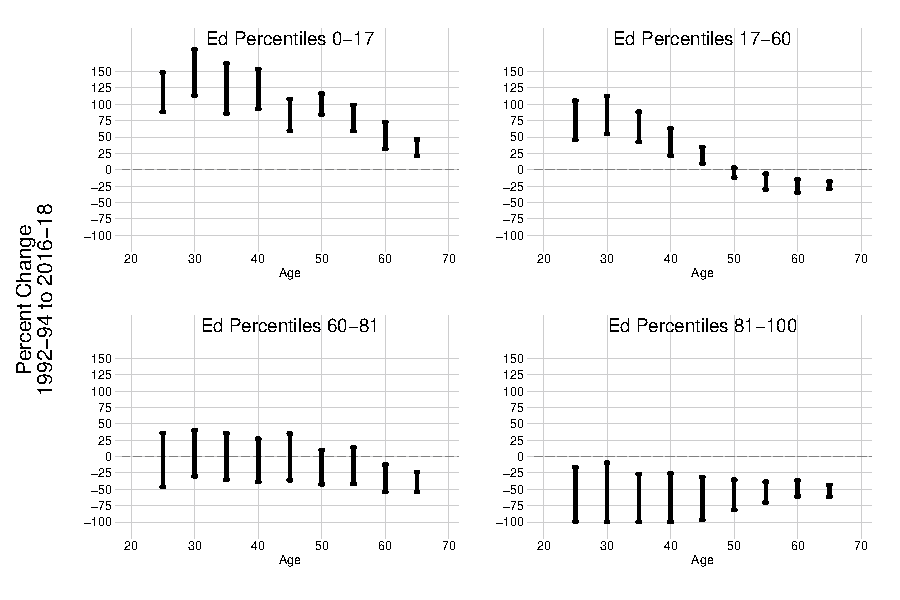
\includegraphics[scale=1.1]{\mortalitypath/causes-1992-2-1} &
  \end{center}

  \begin{center}
    \vspace{-.6cm}
    Panel B: Within Race-Gender Percentiles
  \end{center}
  \vspace{-1.4cm}
  \begin{center}
    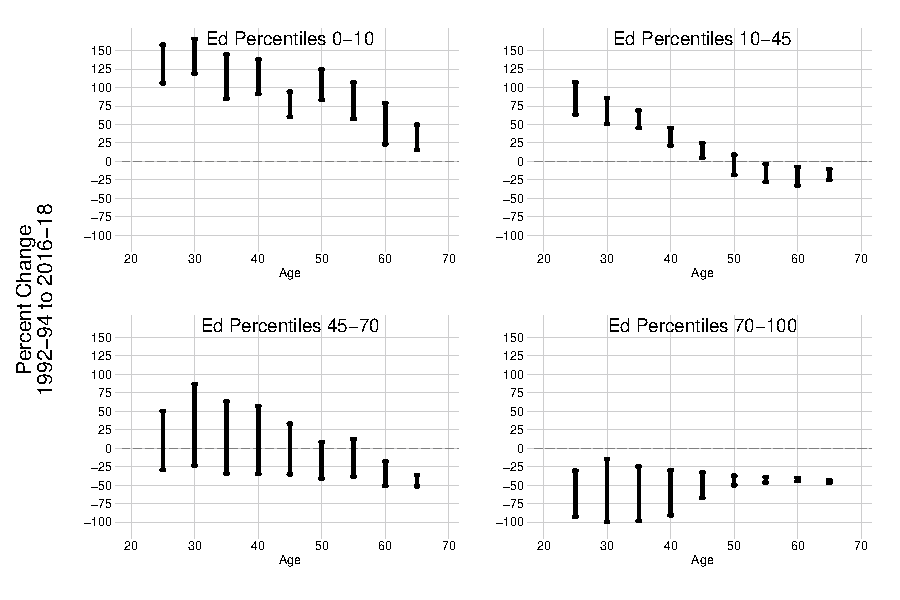
\includegraphics[scale=1.1]{\mortalitypath/causes-racesex-2-1} \\
  \end{center}
\end{figure}

\begin{figure}[H]
  \begin{center}
    \vspace{-.6cm}
    Panel C: Allow Sheepskin Effects
  \end{center}
  %\vspace{-1.4cm}
  \begin{center}
    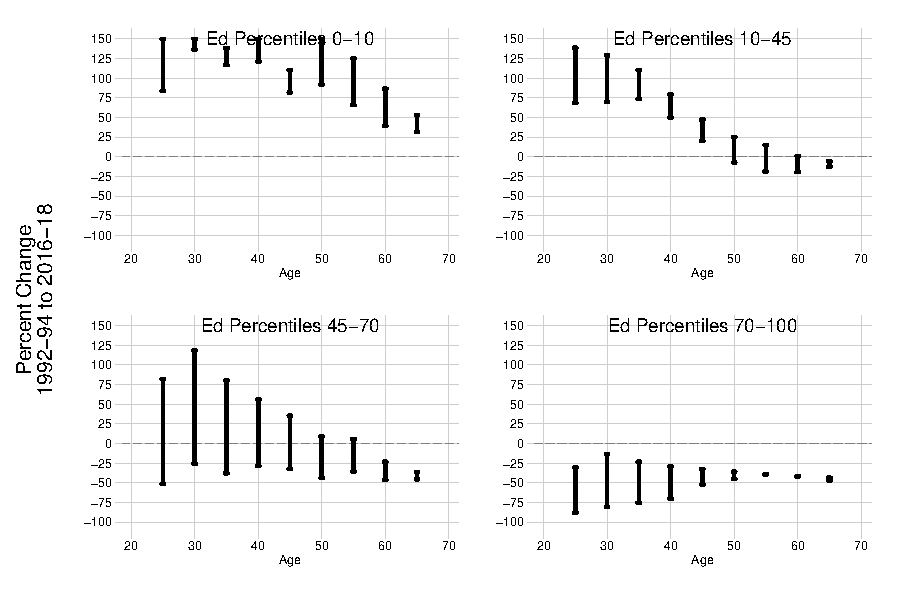
\includegraphics[scale=0.78]{\mortalitypath/causes-mon-step-2-1} &
  \end{center}
  \begin{center}
    \vspace{-.6cm}
    Panel D: No Smoothness Assumption
  \end{center}
  %\vspace{-1.4cm}
  \begin{center}
    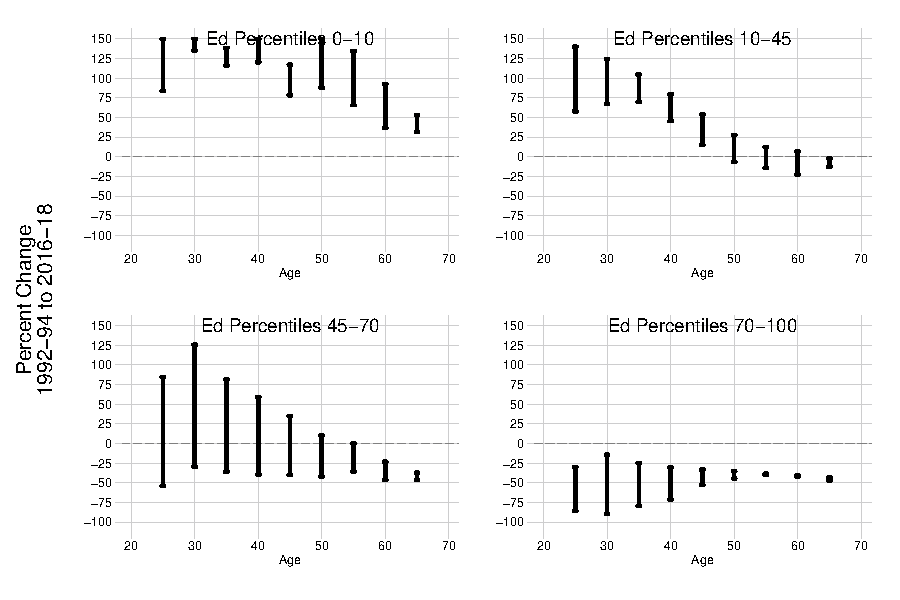
\includegraphics[scale=0.78]{\mortalitypath/causes-nof2-2-1} \\
  \end{center}
\end{figure}
\vspace{-1cm}
\tiny{Note: The figure shows bounds on mortality change from 1992--1994 to 2016--2018, for non-Hispanic white women, by age and percentile education bin, under alternate assumptions from the main body of the paper. The figure is analogous to Panel A of Figure 6, but with different bounding assumptions. Panel A defines education bins boundaries according to education levels in 1992--1994. Panel B defines an individual's education percentile according to the individual's rank in the own-race and own-gender education distribution, rather than in the own-gender education distribution. Panel C allows sheepskin effects, by allowing kinks and discrete jumps at education boundaries (e.g. the rank separating dropouts from high school completers). Panel D estimates bounds on mortality without restricting the curvature of the mortality-education CEF.  The lines show the bounded set containing the percentage change in the mortality rate from 1992--1994 to 2016--2018 for the given group.}

%%%%%%%%%%%%%%%%%%%%%%%%%%
%% Figure: Black Men %% %%
%%%%%%%%%%%%%%%%%%%%%%%%%%
\begin{figure}[H]
  \caption{Sensitivity Analysis: Non-Hispanic Black Men}
  \begin{center}
    \vspace{-.6cm}
    Panel A: 1992 Percentile Boundaries
  \end{center}
  \vspace{-1.4cm}
  \begin{center}
    \includegraphics[scale=1.1]{\mortalitypath/causes-1992-1-2} &
  \end{center}

  \begin{center}
    \vspace{-.6cm}
    Panel B: Within Race-Gender Percentiles
  \end{center}
  \vspace{-1.4cm}
  \begin{center}
    \includegraphics[scale=1.1]{\mortalitypath/causes-racesex-1-2} \\
  \end{center}
\end{figure}

\begin{figure}[H]
  \begin{center}
    \vspace{-.6cm}
    Panel C: Allow Sheepskin Effects
  \end{center}
  %\vspace{-1.4cm}
  \begin{center}
    \includegraphics[scale=0.78]{\mortalitypath/causes-mon-step-1-2} &
  \end{center}
  \begin{center}
    \vspace{-.6cm}
    Panel D: No Smoothness Assumption
  \end{center}
  %\vspace{-1.4cm}
  \begin{center}
    \includegraphics[scale=0.78]{\mortalitypath/causes-nof2-1-2} \\
  \end{center}
\end{figure}
\vspace{-1cm}
\tiny{Note: The figure shows bounds on mortality change from 1992--1994 to 2016--2018, for non-Hispanic black men, by age and percentile education bin, under alternate assumptions from the main body of the paper. The figure is analogous to Panel A of Figure 6, but with different bounding assumptions. Panel A defines education bins boundaries according to education levels in 1992--1994. Panel B defines an individual's education percentile according to the individual's rank in the own-race and own-gender education distribution, rather than in the own-gender education distribution. Panel C allows sheepskin effects, by allowing kinks and discrete jumps at education boundaries (e.g. the rank separating dropouts from high school completers). Panel D estimates bounds on mortality without restricting the curvature of the mortality-education CEF.  The lines show the bounded set containing the percentage change in the mortality rate from 1992--1994 to 2016--2018 for the given group.}

%%%%%%%%%%%%%%%%%%%%%%%%%%
%% Figure: Black Women %% %%
%%%%%%%%%%%%%%%%%%%%%%%%%%
\begin{figure}[H]
  \caption{Sensitivity Analysis: Non-Hispanic Black Women}
  \begin{center}
    \vspace{-.6cm}
    Panel A: 1992 Percentile Boundaries
  \end{center}
  \vspace{-1.4cm}
  \begin{center}
    \includegraphics[scale=1.1]{\mortalitypath/causes-1992-2-2} &
  \end{center}

  \begin{center}
    \vspace{-.6cm}
    Panel B: Within Race-Gender Percentiles
  \end{center}
  \vspace{-1.4cm}
  \begin{center}
    \includegraphics[scale=1.1]{\mortalitypath/causes-racesex-2-2} \\
  \end{center}
\end{figure}

\begin{figure}[H]
  \begin{center}
    \vspace{-.6cm}
    Panel C: Allow Sheepskin Effects
  \end{center}
  %\vspace{-1.4cm}
  \begin{center}
    \includegraphics[scale=0.78]{\mortalitypath/causes-mon-step-2-2} &
  \end{center}
  \begin{center}
    \vspace{-.6cm}
    Panel D: No Smoothness Assumption
  \end{center}
  %\vspace{-1.4cm}
  \begin{center}
    \includegraphics[scale=0.78]{\mortalitypath/causes-nof2-2-2} \\
  \end{center}
\end{figure}
\vspace{-1cm}
\tiny{Note: The figure shows bounds on mortality change from 1992--1994 to 2016--2018, for non-Hispanic black women, by age and percentile education bin, under alternate assumptions from the main body of the paper. The figure is analogous to Panel A of Figure 6, but with different bounding assumptions. Panel A defines education bins boundaries according to education levels in 1992--1994. Panel B defines an individual's education percentile according to the individual's rank in the own-race and own-gender education distribution, rather than in the own-gender education distribution. Panel C allows sheepskin effects, by allowing kinks and discrete jumps at education boundaries (e.g. the rank separating dropouts from high school completers). Panel D estimates bounds on mortality without restricting the curvature of the mortality-education CEF.  The lines show the bounded set containing the percentage change in the mortality rate from 1992--1994 to 2016--2018 for the given group.}



\end{document}
